




Переход $4f^{13}({}^2F^o)6 s^2 \ \to\ 4f^{12}({}^3H_5)5d_{3/2}6s^2$ с длиной волны $\lambda = 410.6$ нм (рис. \ref{fig:Tm}) используется в ЗЗ и ОП, так как является достаточно широким $\Gamma = 2 \pi \gamma = 2\pi \cdot 10.5\, \text{МГц}$. Данный переход не является циклическим, так как существуют иные каналы распада на промежуточные уровни \cite{vlad}, но из-за малого коэффициента ветвления $(3\pm1)\times 10^{-7}$ вероятность выхода из цикла мала \cite{Kolachevsky2007}.


\begin{figure}[h]
    \centering
    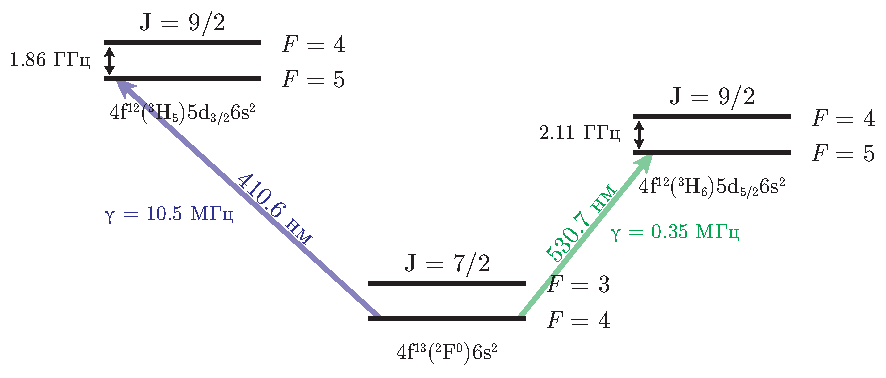
\includegraphics{figs/tm.pdf}
    \caption{Используемые в эксперименте атомные переходы, приведены величины сверхтонкого расщепления \cite{Kolachevsky2007}}
    \label{fig:Tm}
\end{figure}


Переход $4f^{13}({}^2F^o)6 s^2 \ \to\ 4f^{12}({}^3H_6)5d_{5/2}6s^2$ с длиной волны $\lambda = 410.6$ нм (рис. \ref{fig:Tm}) используется в МОЛ, так как имеет более низкий доплеровский предел  $\subt{T}{D} = 8\, \mu\text{K}$. В таблице \ref{tab:tm} приведено большинство параметров для двух охлаждающих переходов. В таблице \ref{tab:tm} содержится естественная ширина линии $\Gamma$, время жизни $\tau$, ширина перехода $\gamma = \Gamma / 2\pi$, интенсивность насыщения $\sub{I}{sat} = \pi h c \Gamma / 3 \lambda^3$, доплеровский предел температуры $\subt{T}{D} = \hbar \Gamma / 2 \kB$, где $h$ -- постоянная Планка, $\hbar = h / 2\pi$, $\kB$ -- постоянная Больцмана, $m$ -- атомная масса.

\begin{table}[h]
	\caption{Некоторые параметры используемых охлаждающих переходов}
	\label{tab:tm}
	\centering
	\begin{tabular}{ll|ll}
	\toprule
	\multicolumn{2}{c}{\multirow{2}{*}{Параметры}} & \multicolumn{2}{c}{Переходы} \\
	&& 410.6 нм &  530.7 нм \\
	\midrule
	Естетсвенная ширина линии & $\Gamma$ (с${}^{-1}$) & $6.6 \times 10^7$ & $2.2 \times 10^6$ \\
	Время жизни & $\tau$ (нс) & 16 & 440 \\
	Ширина перехода  & $\gamma$(МГц) & 10.5 & 0.3455 \\
	Интенсивность насыщения & $\sub{I}{sat}$ (мВт/см${}^2$) & 19.8 & 0.3 \\
	Доплеровский предел & $\subt{T}{D}$ ($\mu$К) & 252 & 8.3 \\
	\bottomrule
	\end{tabular}
\end{table}


% 	